% Chapter 1

\chapter{GAS/DM} % Main chapter title

\label{Chapter1} % For referencing the chapter elsewhere, use \ref{Chapter1} 

%----------------------------------------------------------------------------------------

% Define some commands to keep the formatting separated from the content 
\newcommand{\keyword}[1]{\textbf{#1}}
\newcommand{\tabhead}[1]{\textbf{#1}}
\newcommand{\code}[1]{\texttt{#1}}
\newcommand{\file}[1]{\texttt{\bfseries#1}}
\newcommand{\option}[1]{\texttt{\itshape#1}}

%----------------------------------------------------------------------------------------

\section{}









\section{Figures}


\begin{figure}[h]
\centering
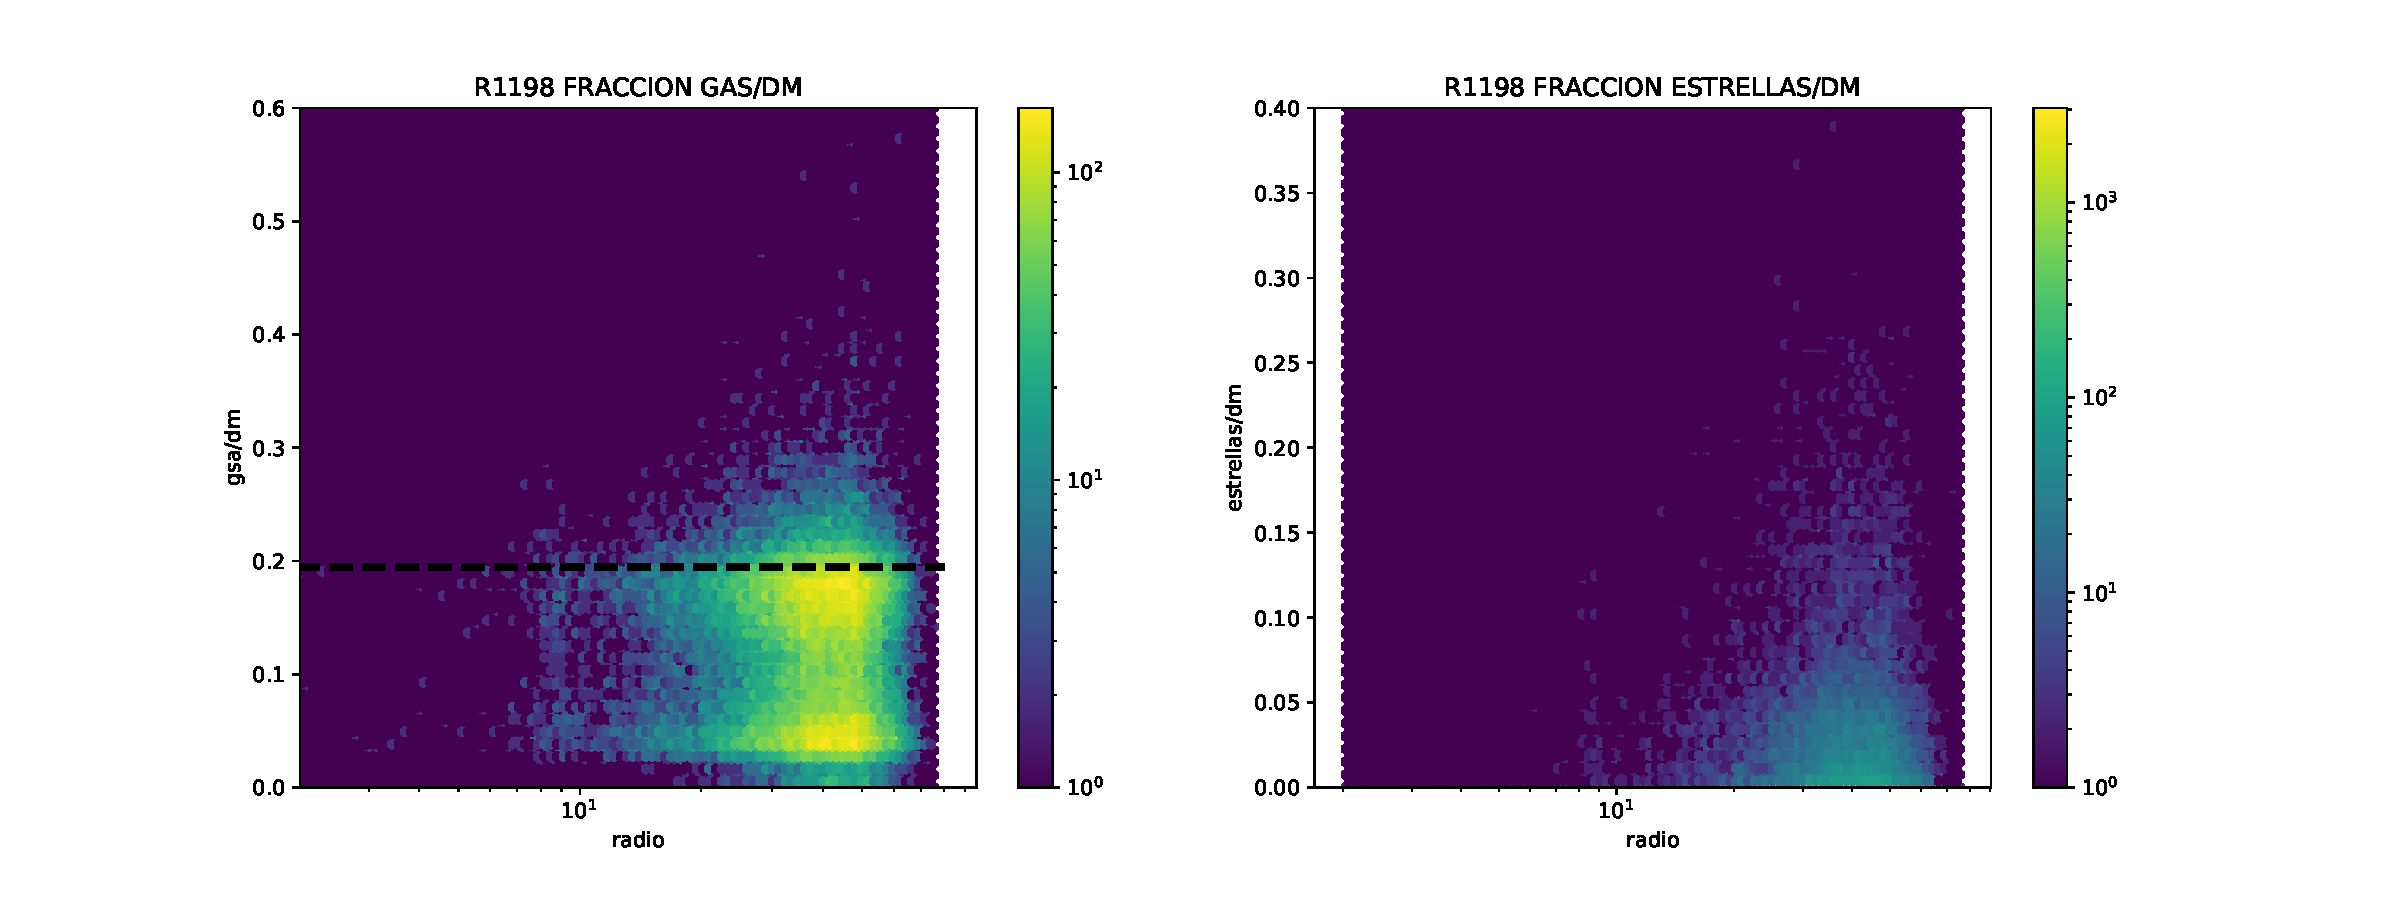
\includegraphics[width=1\textwidth]{Figures/R1198_scatterFRACCIONES.pdf}
\decoRule
\caption[R1198 BARIONES/DM perfil (scatter) ]{Fraccion de gas sobre DM en funcion del centro del void, tamaño del void $\sim$ 9.5 Mpc. A la derecha la fraccion es de Estrellas sobre DM}
\label{fig:Electron}
\end{figure}

\begin{figure}[h]
\centering
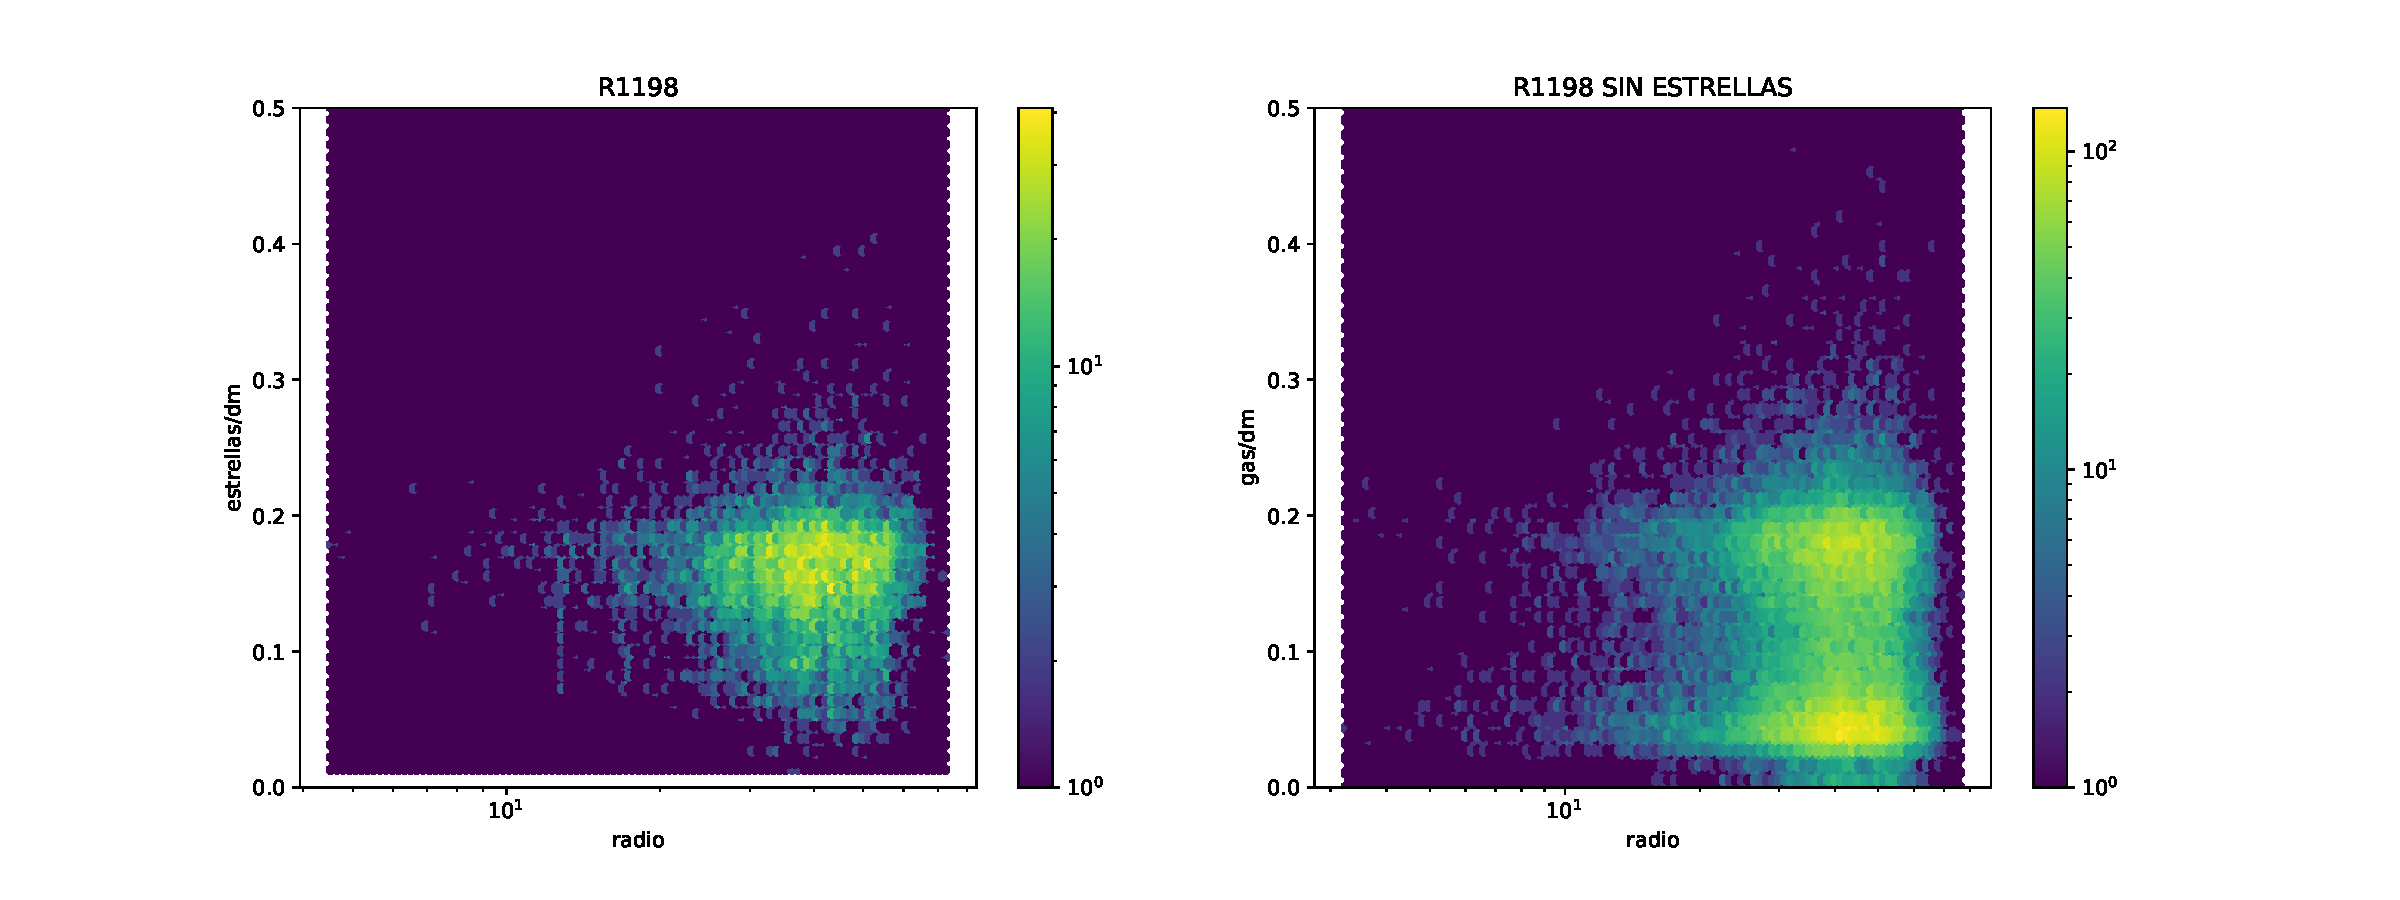
\includegraphics[width=1\textwidth]{Figures/R1198_scatterFRACCIONES_con&sinEST.pdf}
\decoRule
\caption[R1198 GAS/DM perfil (scatter) con y sin estrells]{Perfil de gas/dm para los halos. A  la izquierda estan los halos que contienen al menos una particula de estrellas. A la derehc a los que no tienen ninguna estrella}
\label{fig:Electron}
\end{figure}

\begin{figure}[h]
\centering
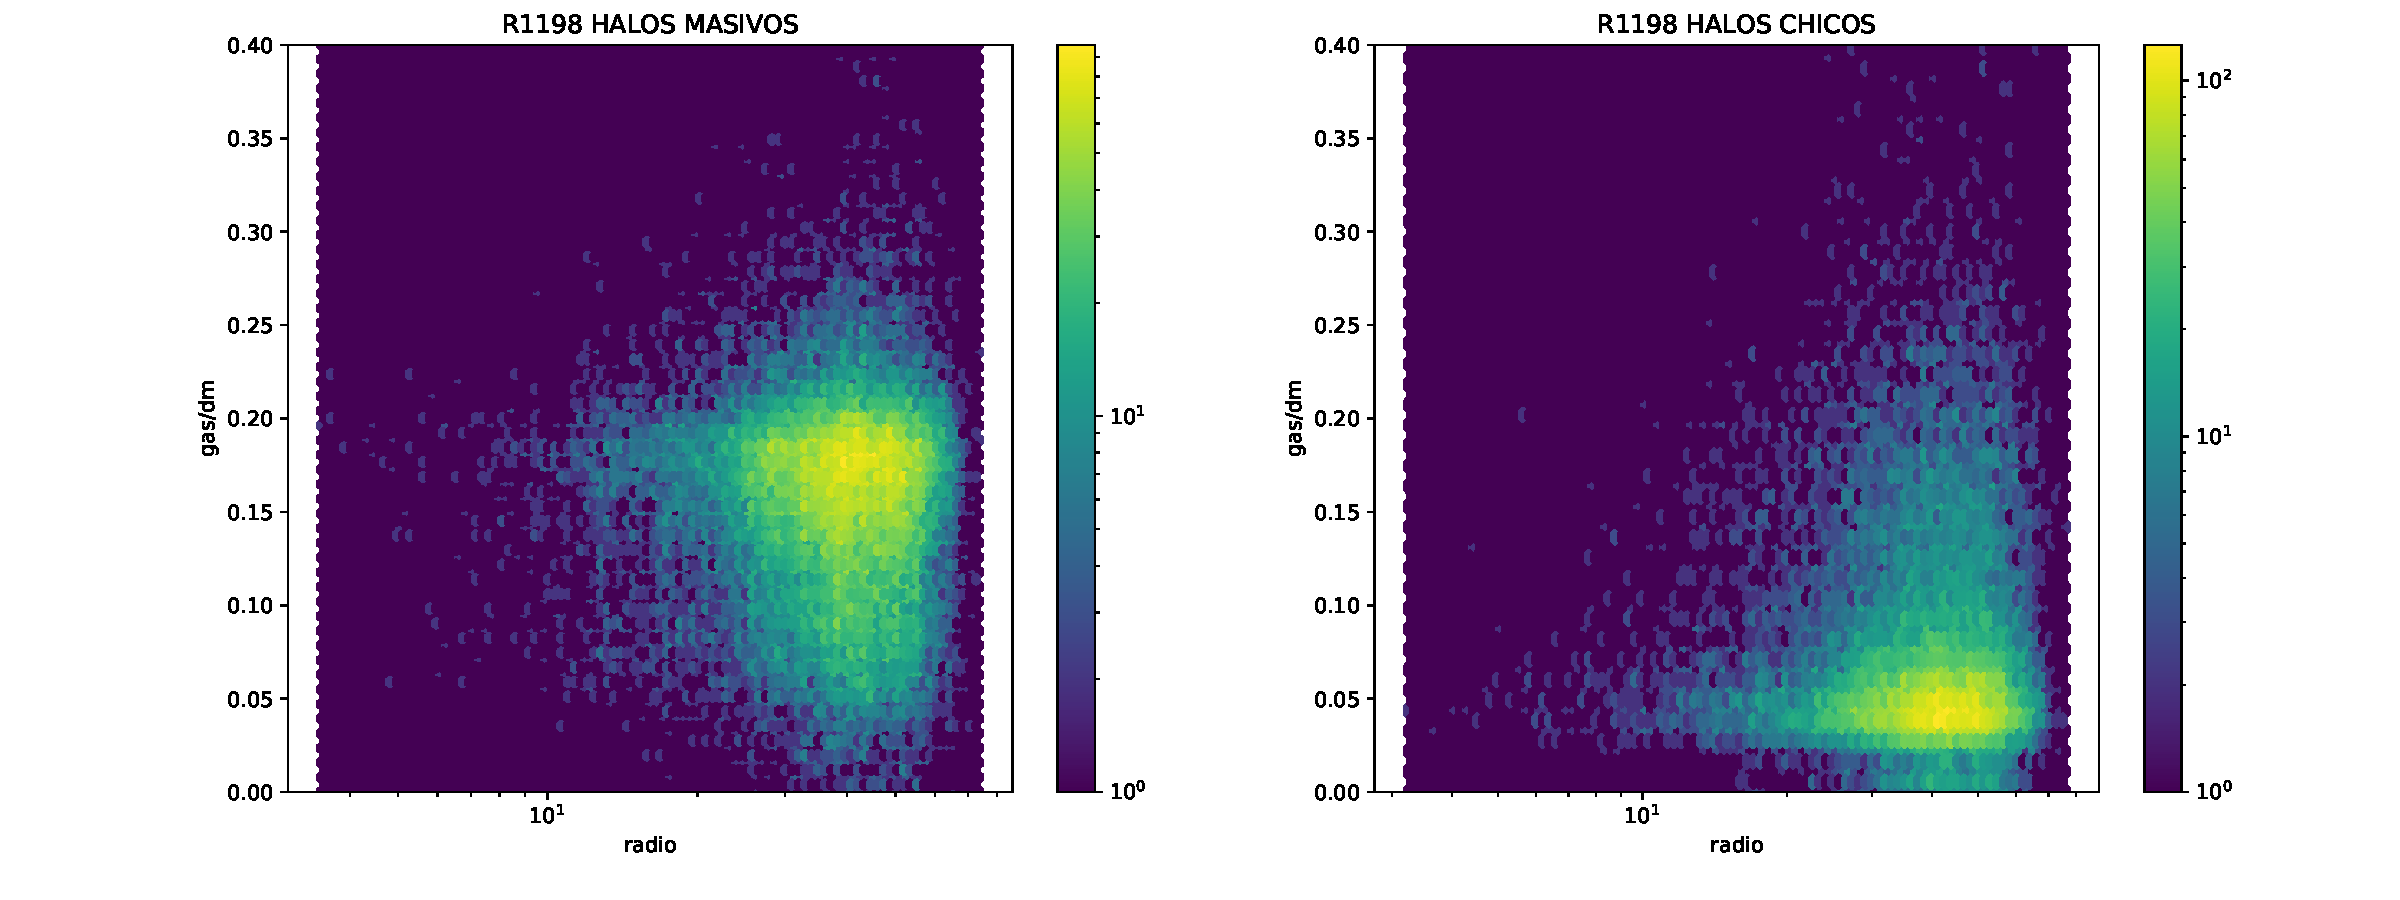
\includegraphics[width=1\textwidth]{Figures/R1198_scatterFRACCIONES_grandesYchicos.pdf}
\decoRule
\caption[R1198 GAS/DM perfil (scatter) halos grandes y chisos]{fraccion de gas sobre DM separando los halos por tamaño. Los halos GRANDES tienen mas de 50 particulas de DM, los chicos menos de 50. }
\label{fig:Electron}
\end{figure}


\begin{figure}[h]
\centering
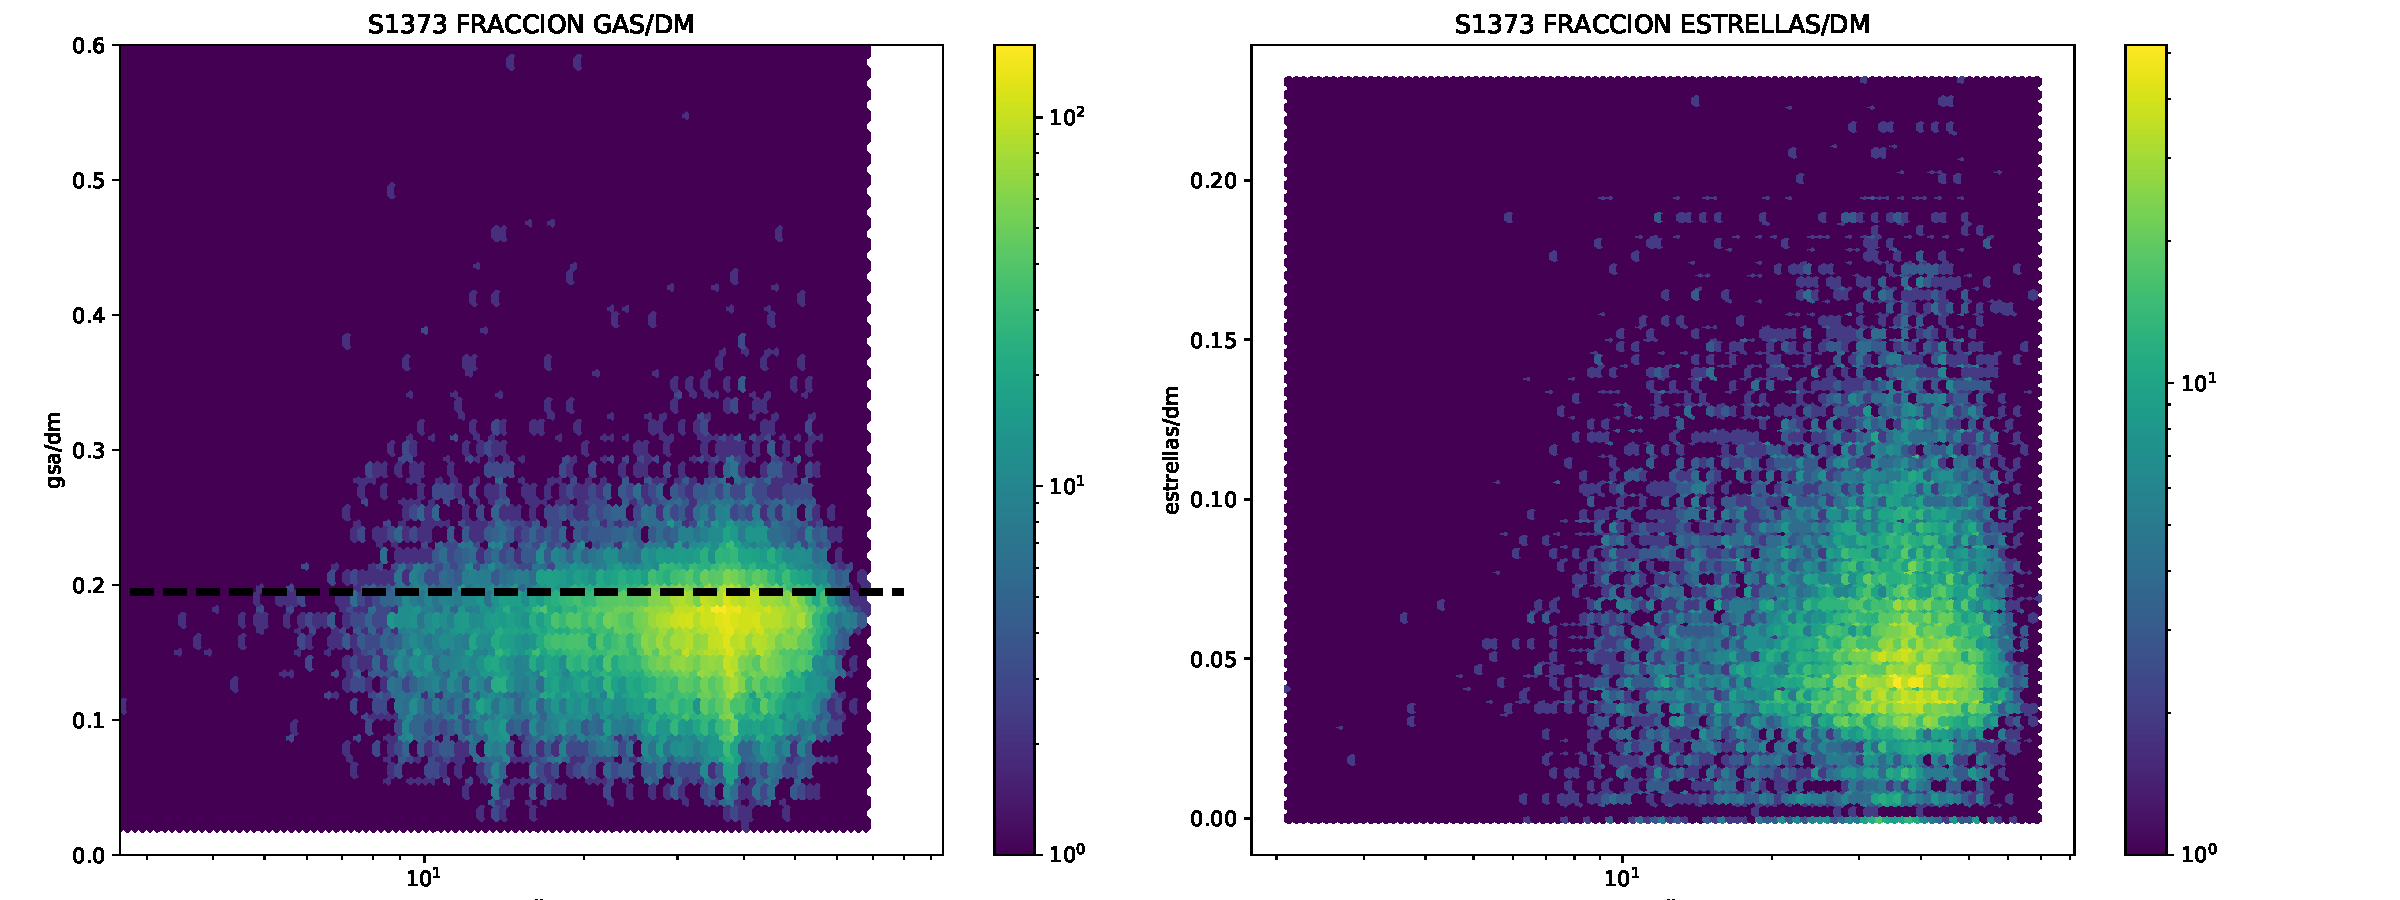
\includegraphics[width=18cm]{Figures/S1373_scatterFRACCIONES2.pdf}
\decoRule
\caption[S1373 GAS/DM perfil (scatter)]{El SPH considera las 32 ? particulas mas cercanas para calcular el hsml, entonces un halo que tenga al menos 32 particulas de gas va a tener sus 23 vecinas en el halo (casi seguro) entonces la masa de gas de ese halo van a ser todas las particulas en el (IZQUIERDA). A unn halos con menos de 32 particulas de gas, le va a pasar que sus particulas de gas van a tener masa FUERA del halo DERECHA).}
\label{fig:Electron}
\end{figure}








\begin{figure}[h]
\centering
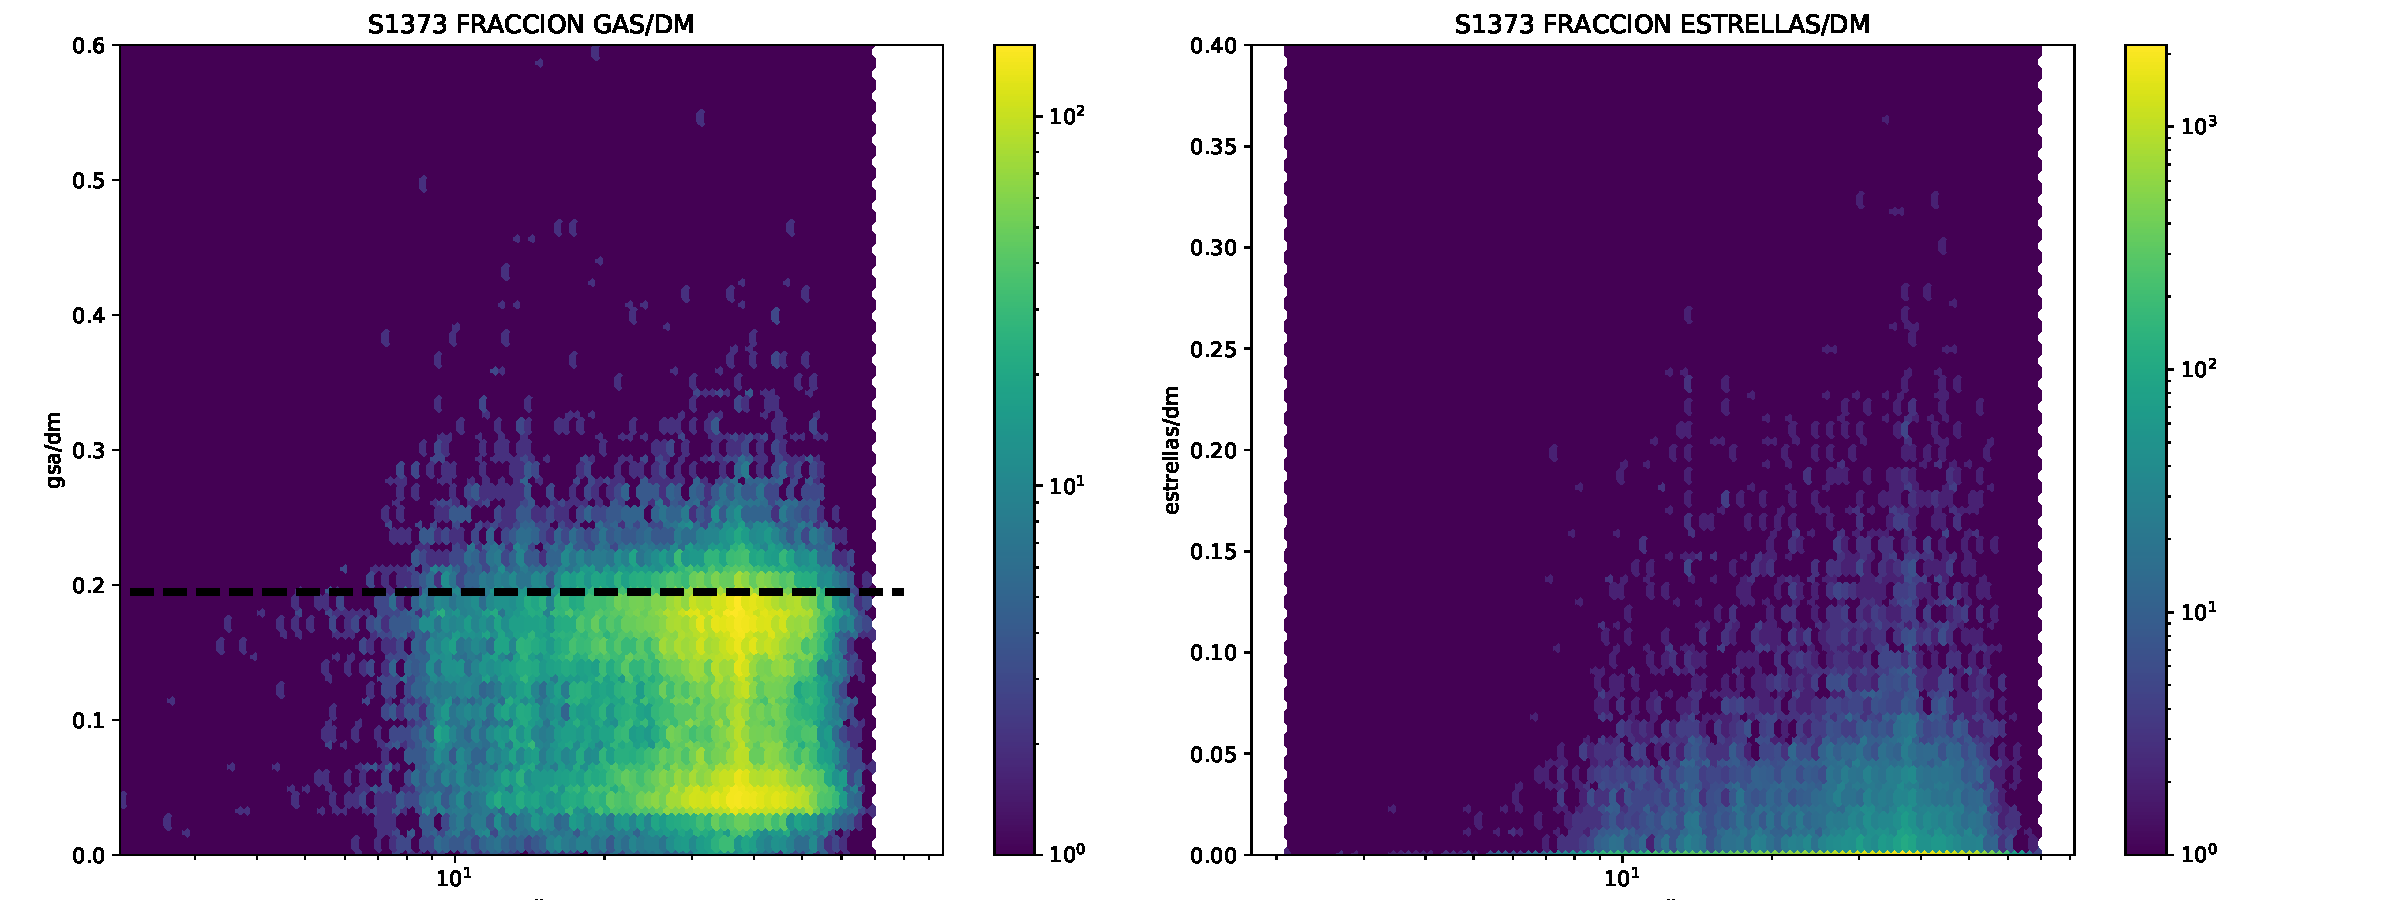
\includegraphics[width=18cm]{Figures/S1373_scatterFRACCIONES.pdf}
\decoRule
\caption[S1373 GAS/DM perfil (scatter)]{Fraccion de gas sobre DM en funcion del centro del void, tamaño del void $\sim$ 9.5 Mpc. A la derecha la fraccion es de Estrellas sobre DM}
\label{fig:Electron}
\end{figure}

\begin{figure}[h]
\centering
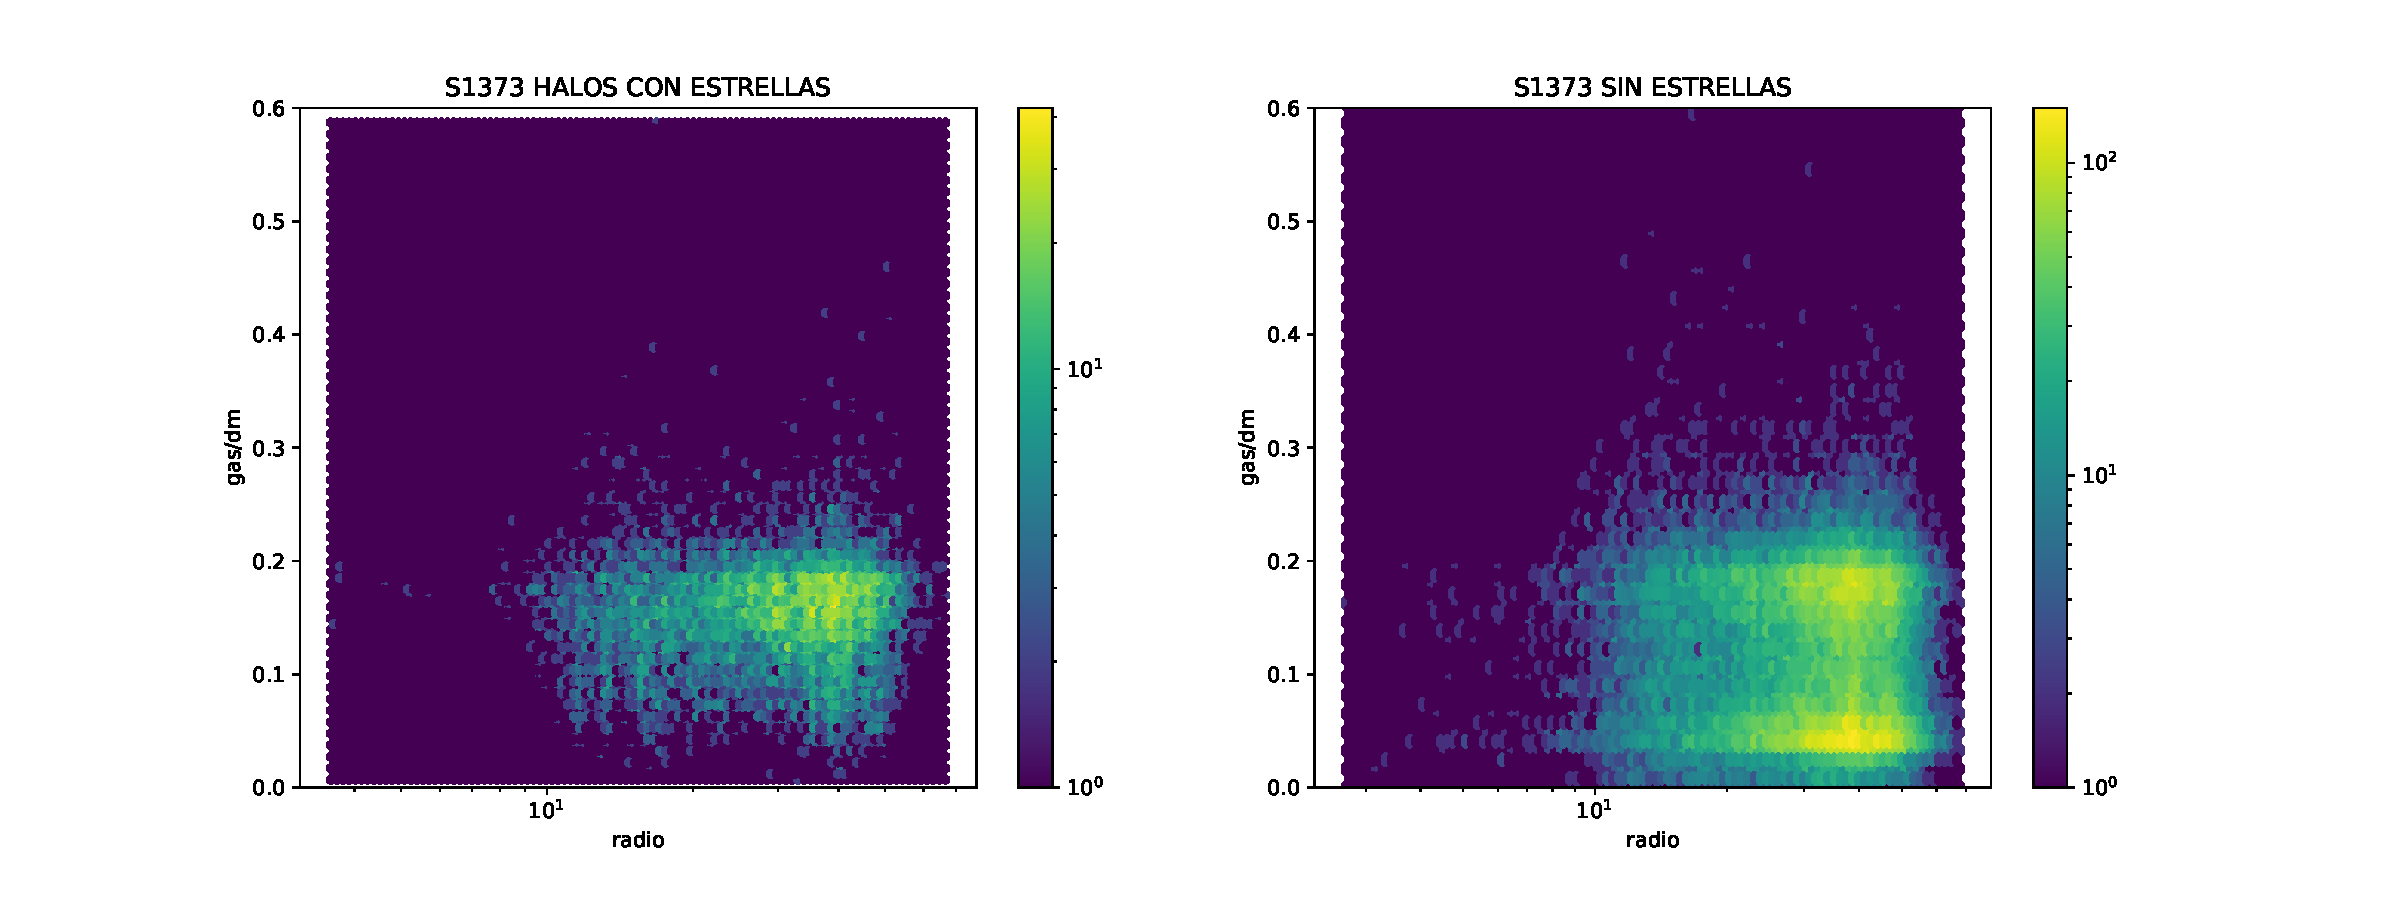
\includegraphics[width=18cm]{Figures/S1373_scatterFRACCIONES_con&sinEST.pdf}
\decoRule
\caption[R1198 GAS/DM perfil (scatter) con y sin estrellas]{Perfil de gas/dm para los halos. A  la izquierda estan los halos que contienen al menos una particula de estrellas. A la derehc a los que no tienen ninguna estrella}
\label{fig:Electron}
\end{figure}

\begin{figure}[h]
\centering
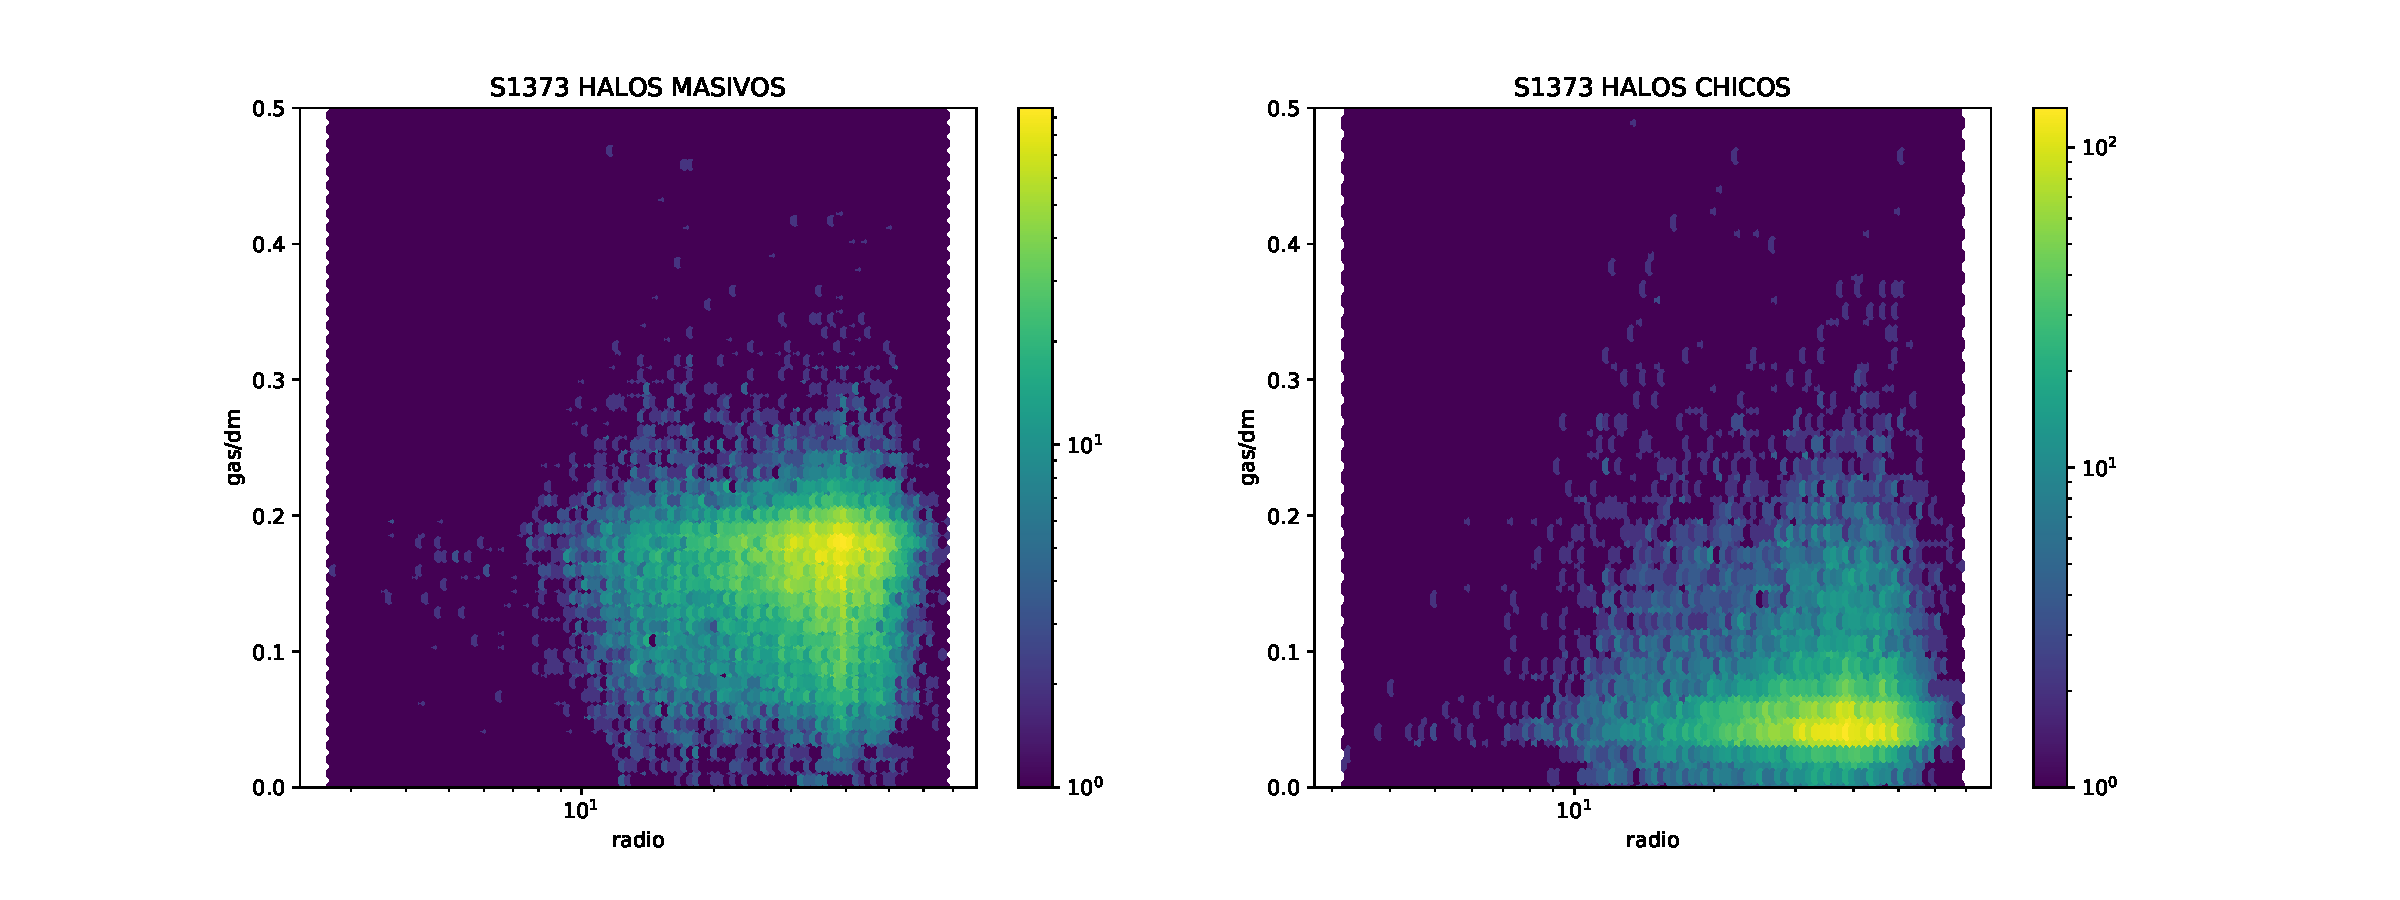
\includegraphics[width=18cm]{Figures/S1373_scatterFRACCIONES_grandesYchicos.pdf}
\decoRule
\caption[R1198 GAS/DM perfil (scatter) halos grandes y chicos]{fraccion de gas sobre DM separando los halos por tamaño. Los halos GRANDES tienen mas de 50 particulas de DM, los chicos menos de 50. }
\label{fig:Electron}
\end{figure}

